\documentclass[oneside,12pt]{discsthesis}
\usepackage{graphicx}
\usepackage{multirow}
\usepackage{fancyvrb}
\usepackage[titletoc]{appendix}
\usepackage{subcaption}
\usepackage{siunitx}
\usepackage{pdfpages}
\usepackage{lscape}
\usepackage{adjustbox}
\usepackage{longtable}
\usepackage{url}
\usepackage{booktabs}
\usepackage{makecell}
\usepackage{setspace}
\usepackage{import}
\usepackage{biblatex}
\addbibresource{references.bib}
\usepackage[a4paper,left=1.5in,right=0.98in,top=1in,bottom=1in,marginparsep=0in,marginparwidth=0pt,headheight=0.5in,headsep=2\baselineskip,footskip=0truein]{geometry}
\pdfoptionpdfminorversion=7

\title{Exploring alternative topologies in a software-defined network quality of service testing framework}
\author{Hyeong Seon Yoo}
\date{March 1, 2022}

\begin{document}
\ThesisAuthor{Hyeong Seon Yoo}
\ThesisTitle{EXPLORING ALTERNATIVE TOPOLOGIES IN A SOFTWARE-DEFINED NETWORK QOS TESTING FRAMEWORK}
\ThesisArea{Computer Science}
\ThesisDefenseYear{2023}
\DefenseDate{April 2, 2023}
\ThesisGrade{}
 
\DepartmentHead{ANDREI D. CORONEL, Ph.D.}
\SchoolHead{EVANGELINE P. BAUTISTA, Ph.D.}
\ThesisAdviser{WILLIAM EMMANUEL S. YU, Ph.D.}
\FirstPanelMember{MA. MERCEDES T. RODRIGO, Ph.D.}
\SecondPanelMember{JOHN PAUL C. VERGARA, Ph.D.}

\ThesisStyle{MS}{Final}{-10pt}{15pt}
  
%% Choices for the 1st argument: MS, PhD
%% Choices for the 2nd argument: Final, FinalWithCorner, Draft

%%\FrontMatter
\begin{thesisabstract}
\paragraph{         }This paper is a sample document that serves as a format and content guideline for undergraduate thesis submissions to the Department of Information Systems and Computer Science. In this section, the abstract, the group should be able to give the readers a clear and concise overview of their study. The section should contain the objectives of the thesis, the methods to be used, and when available, the results of the study, the conclusion, and the recommendations for further work, all based on the intended research objectives. A good abstract should be at most around 150-200 words, or half a page. It should also not contain any references, figures, or equations.
\end{thesisabstract}

\begin{acknowledgments}
\noindent Deepest gratitude to Dr. William Emmanuel S. Yu, my research adviser, for his excellent advice and guidance for accomplishing this thesis. Dr. Yu has been a great mentor who enabled me to go beyond and achieve excellent results. Without his guidance, this paper would not have been possible.

Many thanks to Dr. Andrei D. Coronel and Jessica O. Sugay for their invaluable insights, suggestions, and advice as panelists. They have greatly improved the quality of this research, and gave me encouragement to pursue excellence.

I would also like to thank my colleagues, Aldrich Ellis C. Asuncion, Brian Christopher T. Guadalupe, Raphael Jose Montemayor and Christopher William S. Dizon for their practical advice in the process of accomplishing this thesis.

To my family, many thanks for their continued support in my pursuit of academic excellence in Ateneo.

And finally, praise be to God, whose infinite love provides all things graciously, including this thesis.
\end{acknowledgments}
\tableofcontents
\listoffigures
\listoftables


\chapter{INTRODUCTION}

\section{Context of Study}

Network demands for video-conferencing and other high-bandwidth technology is becoming more complex, as well as the network infrastructure that support these demands. For this reason, it is important to develop and test good Quality of Service (QoS) methods, not only in model, typical networks but also in real-life networks. QoS refers to technology that guarantee high-quality provision of resource-intensive, high-priority services \cite{noauthor_what_nodate}. Requirements of QoS are enforced through queuing, which is the ordering of packets in traffic flow, and bandwidth control, which is how much of the network resources the packets take up \cite{zhao_internet_2000}. In traditional networks with disparate forwarding devices with different configurations, queuing and bandwidth control is enforced through service-level agreements between the user and the network provider \cite{karakus_quality_2017}. This does not allow for abstract and fine-grained control of network traffic.

Software-defined networking (SDN) is an emerging network architecture that solves the problem of fragmented network management and configuration by decoupling the data plane from the control plane \cite{kreutz_software-defined_2015}. Forwarding devices in the network are logically centralized, and uses a protocol such as OpenFlow to control behavior. Software-defined networking allows for QoS provisioning to be implemented with a more abstract view of the network, allowing for better control of different types of traffic. Advantages of the SDN paradigm in providing SDN include custom routing of QoS traffic instead of shortest-path routing, better QoE through additional parameters to the traditional QoS metrics, and better monitoring of network dynamics.

Researchers have tested many QoS algorithms on Mininet, which simulates software-defined networks, with a network operating system such as Ryu and OpenFloodLight \cite{karakus_quality_2017}. Regencia and Yu built a testing framework with Mininet and Ryu to test various QoS algorithms under different network topologies \cite{yang_introducing_2022}. However, the study did not investigate the performance of those QoS algorithms in different topologies. The QoS algorithms can be more thoroughly tested with real-world data from the Internet Topology Zoo (ITZ) \cite{knight_internet_2011}, which provides data from network operators about live networks that provide Internet service. This testing is important so that the characteristics of the performance of the different algorithms to understand which are the most optimal in real-world network use cases. It also take full advantage of the flexibility of configuration brought by Software-defined networks, which allow control of the nodes and switches in the network without the constraints of hardware-bound firmware control of traditional networks. Note that there are other networking use cases such as QoE and security that can be applied to this framework of testing, especially with different topologies.

\section{Research Objectives}
The main objective of this study is to analyze Class-based QoS algorithm performance in various network topologies. To achieve this, we modified the aforementioned framework which has been written to generalize layers in a fat-tree topology to generalize for a general graph topology. In that process, we expect to find some differences in network behavior and they can be quantified. Hence, we have the following specific objectives:

\begin{enumerate}
    \item Modify the framework by Regencia and Yu to easily simulate various network topologies and QoS algorithms in those topologies,
    \item Analyze performance of QoS Techniques in different network topology with synthetic traffic load,
    \item And find differences in behavior of the different network topologies, quantify them, and resolve issues that might arise from those differences.
\end{enumerate}

\section{Research Questions}
In this study, we investigate the performance of QoS provisioning algorithms over different network topologies, especially in live network topologies from the ITZ. We aim to answer the following questions:

\begin{enumerate}
    \item How well do Class-based Queuing QoS techniques perform under different network topologies?
    \item What are the differences in the performance characteristics of the different QoS techniques?
    \item Which QoS techniques exhibit the best performance in the different network topology tested?
\end{enumerate}

These research questions were modified since the start of this study, for the reason that the analysis of core-enforced queuing versus leaf-enforced queuing was not completed during the period given for this study.

\section{Scope and Limitations of the Study}

We test the following topologies in the research:
\begin{itemize}
    \item Fat tree with fanout of 3 and 2 layers,
    \item Complete mesh network with 5 Openflow switches,
    \item Networks from data provided by the Internet Topology Zoo.
\end{itemize}

For networks from data provided by the Internet Topology Zoo, We select regional and country-level data with at most 40 nodes to ensure that we have sufficient computing resources for the simulation under the heavy synthetic simulations that will be maintained from the previous study. Only 110 topologies with 40 nodes or less, out of 212 regional/country-level data from the dataset. 

Only the topology connecting the clients was from the study by Regencia and Yu. The network traffic tested will be HTTP requests for images and PDF files, and video-on-demand through the VLC Media Player RTSP servers and clients.
    
We also limited the tested QoS algorithms to the following:
\begin{itemize}
    \item Basic Class-Based Queuing, leaf-enforced
    \item Source Class-Based Queuing, leaf-enforced
\end{itemize}

In testing the topology from the Internet Topology Zoo, we assume that all connections are the same, because metadata on the links between the nodes are not present for all nodes.

\section{Significance of the Study}

This is an extension of the framework introduced by Regencia and Yu in testing QoS algorithms. Since network infrastructure is varied across different places and applications, testing QoS provisioning techniques over various topology will provide better insight to how the techniques perform in real-life contexts. Results of this research can further enable research into finding better QoS routing and queuing techniques by identifying the characteristics of each technique over different topologies. The framework for analyzing various network topologies can be further used in network design and testing new algorithms. Finally, the research will allow network providers to implement better techniques for QoS in providing resource-intensive and critical network traffic such as video conferencing and video-on-demand.


\chapter{REVIEW OF RELATED LITERATURE}

\section{Software Defined Networking}
Software-defined networking (SDN, also refers to \textit{software defined networks}) is a networking architecture that arose due to the need for a centralized control, programmability and automation in a network \cite{open_networking_foundation_software-defined_2013}. In traditional networks, fulfilling this requirement meant specific control of different forwarding devices in the network, each with its own control plane (deciding how to handle network traffic) and forwarding plane (forwarding traffic according to the decisions made by the control plane) \cite{kreutz_software-defined_2015}. To solve this, SDN separates the forwarding plane from the control plane, and introduces the concept of a logically centralized \textit{controller} \cite{open_networking_foundation_software-defined_2013}. In this model, network devices simply become forwarding devices which receive instructions from the controller on how it treats different types of network traffic. Network applications such as traffic engineering, monitoring and security such as firewalls can interact with the controller, instead of the network itself \cite{kreutz_software-defined_2015}.

\section{OpenFlow and OpenFlow-based SDN Controllers}
OpenFlow is a protocol that allows controllers to communicate with forwarding devices in a standardized way, first proposed by McKeown et. al. \cite{mckeown_openflow_2008}. In OpenFlow, instructions on incoming traffic is \textit{flow-based}. A \textit{flow} is a sequence of packets from a source to a destination, which receive the same treatment at forwarding devices. The controller controls all of these flows; therefore, the controller an is an abstraction of the underlying network. OpenFlow consists of message types that control the behavior of forwarding devices (in this case, \textit{OpenFlow switches}), and message types that where forwarding devices tell the controller about the its own status \cite{open_networking_foundation_openflow_2009}. The \textit{Secure channel} connects the controller to OpenFlow switches, and all OpenFlow messages are sent through this channel. When an OpenFlow switch encounters a packet, it sends a \textsc{Packet-In} message to the controller. The controller then instructs the switch that sent the message to perform some \textit{action} on the packet. This action can be dropping a packet, forwarding a packet to a port, or making modifications to the data before forwarding the packet. Additionally, the controller can send a \textit{Flow-Mod} instruction that allows the OpenFlow switch to remember in its \textit{Flow Table} the action/s taken on packets that \textit{match} certain characteristics \cite{open_networking_foundation_openflow_2009}. In summary, the role of the OpenFlow controller is to instruct the forwarding devices on how to treat incoming network traffic.

The controller is implemented as \textit{software} that manages the network devices. Examples of OpenFlow controllers include  POX, OpenDaylight, Floodlight and Ryu \cite{salman_sdn_2016}. POX was used in Pena and Yu \cite{pena_development_2014} to successfully implement a distributed firewall, with testing done in Mininet, a testbed for simulating realistic networks in a single machine \cite{noauthor_mininet_nodate}. This thesis used Ryu because it is relatively well documented among the Python-based controllers \cite{salman_sdn_2016}. Ryu is an open source framework that provides basic controller functionality for SDNs. Ryu facilitates an SDN application development, and supports a wide range of the OpenFlow specifications, making it appropriate for the development of network applications \cite{kubo_ryu_2014}. 


\section{Quality of Service}
Quality of Service(QoS) is a set of technologies aimed at providing a certain level of guarantee to resource intensive or performance sensitive traffic flow from important applications such as VoIP, video conferencing, and online gaming. Metrics used to assess QoS include delay, bandwidth, jitter, and packet loss \cite{karakus_quality_2017}. The two largest QoS architectures in traditional networks are IntServ and DiffServ. IntServ works by the individual routers reserving a portion of resources with the Resource Reservation Protocol in order to provide quantifiable QoS per flow \cite{braden_rfc1633_1994}. While this allows for exact control of QoS guarantees, it requires that all routers support the protocol, which means that it will not scale well. DiffServ works with aggregated classes of IP packets based on the Differentiated Service Code Point (DSCP) field to change the Per-Hop Behavior (PHB), which describes how each packet is treated per forwarding device, usually relative to other PHBs \cite{blake_rfc2475_1998}. While DiffServ allows for better scalability and simpler configuration, it leaves control policy as a separate issue, therefore it is harder to have finer-grain control \cite{zhao_internet_2000}.


\section{QoS Provisioning and Management in SDN}
The previous examples of IntServ and DiffServ show that configuring disparate devices is not suitable to meet the constantly changing demands of QoS. Software-defined networking alleviates this problem by providing a logically central point of control that can abstract the network into a consistent API that network applications can work with \cite{kreutz_software-defined_2015}. Because of this, QoS Provisioning with Software-defined networking has been an important topic of research in the last decade, with many attempts to simulate various conditions and QoS provisioning methods over different platforms and environments.

QoS Routing is a basic problem of QoS Provisioning where the paths that packets take need to satisfy a wide range of QoS constraints \cite{zheng_wang_quality--service_1996}. SDN enables for more sophisticated methods of routing based on QoS parameters, instead of defaulting to the shortest path routing. Kuipers and Van Mieghem \cite{goos_qos_2001} provided an exact algorithm that guarantees to find a path that satisfies QoS constraints, if it exists, and tested the algorithms on random graphs. Kaiming and Liu \cite{kaiming_liu_novel_2016} introduced a new algorithm to find QoS routing paths in SDN based wireless mesh networks. They used heuristics to solve a NP-Hard problem by dynamically updating weight based on delay and packet loss rate and tested it on Mininet-Wifi with 10 routers and 8 clients.

SDN also enables queue management through the use of OF-CONFIG \cite{bansal_-config_2014} and OVSDB (OpenVSwitch Database) \cite{pfaff_rfc_2013} protocols. Queues are used to shape traffic and limit their bandwidth usage, thereby dividing the resources of the network among different types of traffic. Yan, Zhang, Shuai, Liu and Guo used a combination of multi-path routing and queue separation for different types of traffic to achieve better performance in throughput and resilience \cite{yan_hiqos_2015}. They use Mininet and Floodlight to simulate a relatively simple 5-node, topology with 11 clients and 2 servers. Sudiharto et. al. used a VoIP network setting to compare class-based queuing and priority queuing \cite{sudiharto_comparative_2015}. They used the NS-2 simulator to simulate a topology with 3 servers and 3 clients to find that class-based queuing was the more effective method. Ishimori, Farias, Cerqueira and Abelem used the Stochastic Fairness Queuing technique instead of the First-in-first-out technique to improve Quality of Experience \cite{ishimori_control_2013}. However, the test were limited to the single-switch topology and the linear topology. Chato and Yu investigated different class-based queuing (CBQ) techniques enforced on the core and on the leaves, but experiments were limited to a 3-switch tree topology \cite{chato_exploration_2016}.

\section{QoS and Network Topology}
Different network topologies have different applications, strengths and weaknesses. Mesh networks, for example, are used to maintain reliable and self-healing connections throughout the network \cite{chawla_fault_2015}. Ring networks are used mostly in local area networks where connection is maintained even if one node fails, and since each node has two neighbors, routing is simple. The tree topology is suitable for large geographical areas and thus can be implemented for large-scale networks such as Metropolitan Area Networks \cite{gerla_tree_1988}. Hypercube networks are commonly used in parallel computing applications for inter-networking multiple processors each with their own memory modules \cite{yan_fundamentals_2009}.

While QoS provisioning research as shown in Section 2.2 focused on QoS provisioning, they did not test these techniques in different topologies, especially live networks. However, some work has been done in evaluating QoS techniques and characteristics in different topologies. Guck, Bemten, Reisslein, and Kellerer \cite{guck_unicast_2018} tested many QoS Routing techniques in ring topologies and grid topologies with different sizes. They considered shortest-path and constrained shortest path algorithms for routing, and concluded that different routing algorithms are the best for different topology configurations. Laassiri \cite{laassiri_evaluation_2017} evaluated packet loss, gigue, latency, and end-to-end delay in star, ring, tree, and hierarchical topologies in an SDN network. Regencia and Yu was able to generalize the simple three-node tree topology in the aforementioned study from Chato and Yu to complete binary trees with up to 6 layers \cite{yang_introducing_2022}.

\section{Testing various QoS queuing techniques in SDN}
Community-driven open-source Network Operating System (NOS) software such as Floodlight, NOX, POX, and Ryu have been used in research for testing and simulation purposes. Karakus and Durresi lists research regarding QoS that used Mininet with NOS software to simulate their algorithms \cite{karakus_quality_2017}, such as the aforementioned study by Ishimori et. al. \cite{ishimori_control_2013} and the study by Yan et. al. \cite{yan_hiqos_2015}. Regencia and Yu \cite{yang_introducing_2022} presented a Mininet and Ryu based framework for simulating various QoS queue management algorithms based on the aforementioned previous work by Chato and Yu \cite{chato_exploration_2016}. Torres, Regencia and Yu \cite{kim_real_2021} extended the framework to simulate real-world traffic data from PCAP files. Network testing in these studies were conducted with various traffic generation tools such as Iperf (as in \cite{yan_hiqos_2015} and \cite{ishimori_control_2013}, or ApacheBench and VLC (as in \cite{chato_exploration_2016} and \cite{kim_real_2021}) to load the network with random or synthetic traffic.

\section{Current QoS Testing Framework from Regencia and Yu}
The framework by Regencia and Yu \cite{yang_introducing_2022} accepts custom QoS algorithms and custom parameters for a tree topology as input to a Ryu controller that implements a Level 2 learning switch. Clients, servers, and OpenFlow switches are simulated by Mininet. In the experiment using this framework, the clients configured by the framework continuously make HTTP and VLC video-on-demand requests as synthetic load to the network for 5 minutes. The simulator script launches the benchmarking software within the clients, and the Ryu SDN Controller serves as the controller to the simulated network. Figure \ref{fig:original_architecture} shows the architecture of this testing framework. This is the framework that this thesis intends to build and improve upon.

\begin{figure}[htbp!]
    \centering
    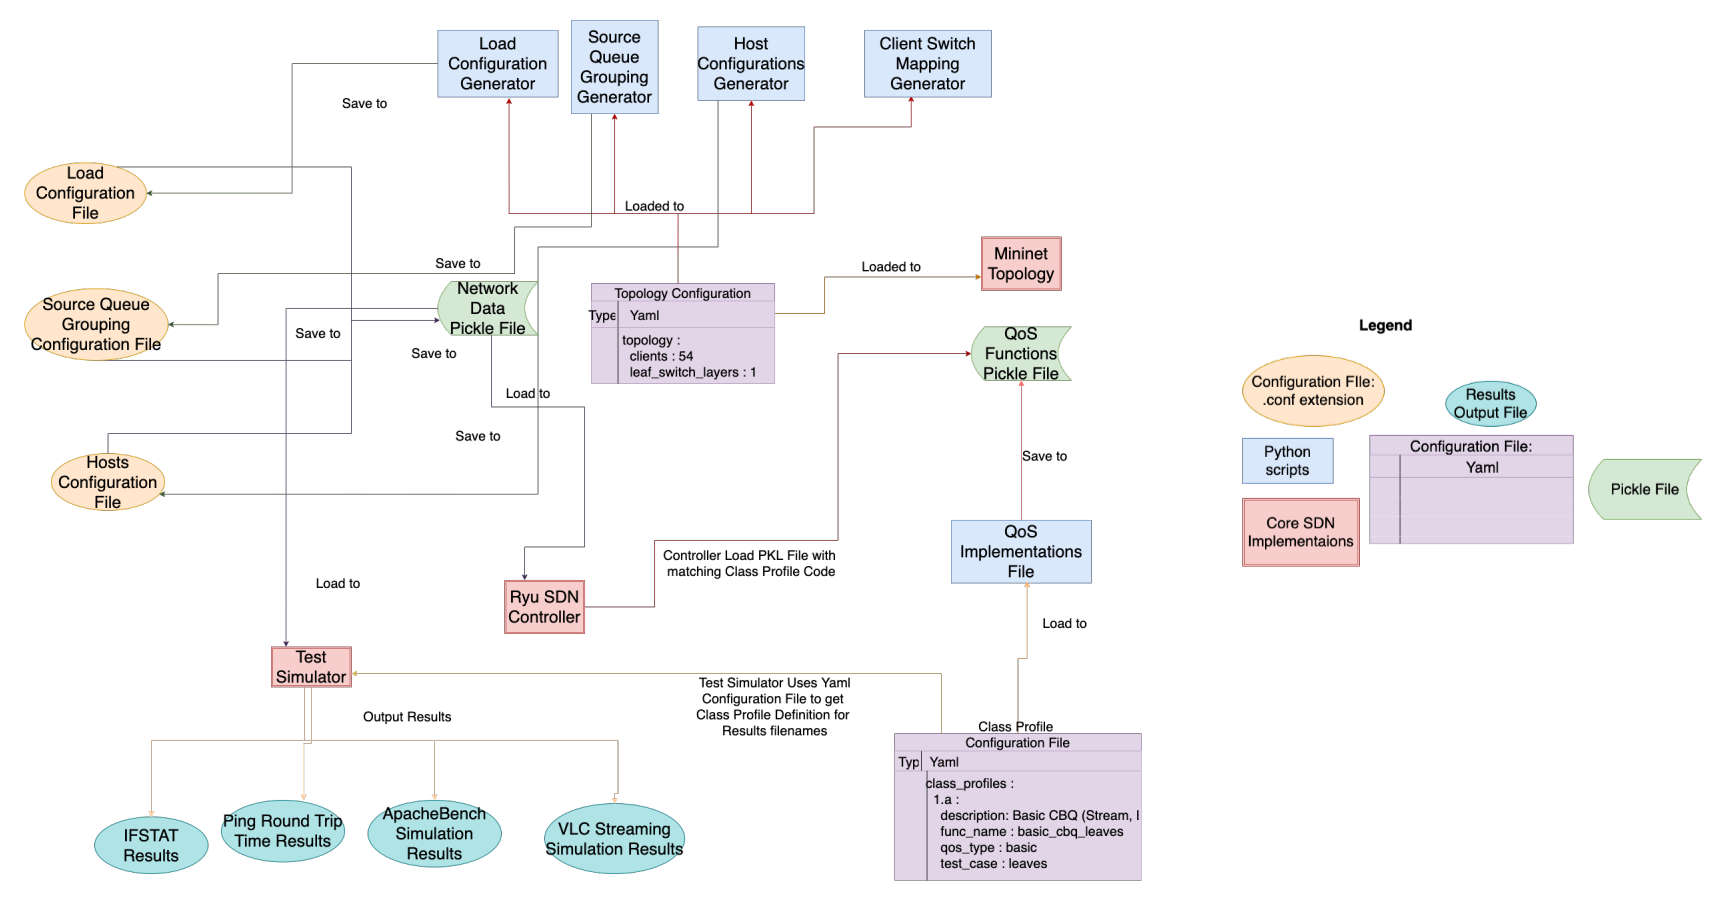
\includegraphics[width=\textwidth]{Figures/original_architecture.png}
    \caption{The architecture of the QoS Testing Framework}
    \label{fig:original_architecture}
\end{figure}

In this architecture, tests are configured with the \textit{Topology Configuration} file and the \textit{Class Profile Configuration File}. These contain the metadata of the network setup of the simulation, as well as the QoS queueing system to be used during the simulation. The metadata are loaded into scripts that generate Python-readable files for use in Mininet, Ryu, and a Python script for automating the execution of the test. The Python-readable files consists of the \textit{Load Configuration}, \textit{Source Queue Grouping Configuration}, and \textit{Hosts Configuration} files. Load Configuration is a list of clients and the requests that the client will make to the servers when running the tests. Source Queue Grouping Configuration contains the switches in the path from the client to a server. Hosts Configuration contains the basic information of each client and server, including the name, IP address, the connected switch, and protocols served.

\section{The Internet Topology Zoo in SDN Research}
The Internet Topology Zoo is a collection of network topologies traced from data provided by network operators around the world \cite{knight_internet_2011}. Some work was done with the Internet Topology Zoo (ITZ) as test data to simulate live networks. Mamushiane, Mwangama, and Lysko \cite{mamushiane_given_2018} test solutions to the placement of controllers in an SDN topology in ITZ data. Metter et. al. also used ITZ data to test the impact of network topology in the processing times of SDN controllers. \cite{metter_investigating_2015}. ITZ data is considered reliable because although it may not represent the networks exactly as running, it represents the network as the company providing the data intended to build. \cite{knight_internet_2011}

\section{Conclusion}
The reviewed literature shows that is important and necessary to test network algorithms in real-life situations, because real-life networks have complex topologies with multiple loops and many switches. There were no significant efforts to test QoS \textit{queuing techniques} in real-life topologies, which is a gap in the literature that this thesis aims to bridge. Since the framework from Regencia and Yu was intended to test different QoS algorithms in many situations, we can modify it to include ITZ data, which will allow for easier and better testing of simple and complex QoS techniques. This thesis will then bridge the aforementioned gap, as Guck et. al. \cite{guck_unicast_2018} was able to do with QoS \textit{routing} algorithms.


\chapter{METHODOLOGY}
\section{Modifying the Testing Framework}
The framework of the study is divided into two parts. First, we expand the QoS Testing Framework (hereby referred to as the \textit{simulator}) from Regencia and Yu to support different classes of topologies: fat-tree topologies with fanout greater than 2, some typical topology shapes, general graphs, and data from the Internet Topology Zoo that follow the constraints in section 1.5. Second, we simulate artificial network load with the same methodology as the Regencia and Yu study onto the newly implemented topologies with the same queue management algorithms. 

To accomplish this, we modify the way the \textit{topology configuration} file is read in the Framework. In the original Framework, the topology configuration file contains information about the number of clients and the number of layers in a tree topology, which is then used by each of the \textit{configuration generator} files to reconstruct the topology within itself to generate the correct configuration (Figure \ref{fig:original_architecture}). 

We modify the Framework such that an intermediary script called the \textit{Topology Information Generator} contains the implementation of the topology (Figure \ref{fig:new_architecture}). The Topology Information Generator then can emit a Topology Information file that can be read by the configuration generators to generate the necessary configuration files. For typical topologies such as fat-trees, mesh, and rings, the implementation of the topology is directly in the topology information generator. For topologies from the Internet Topology Zoo data, the generator parses a GraphML file with the  \textsc{NetworkX} library to generate the same information file.

\begin{figure}[htbp!]
    \centering
    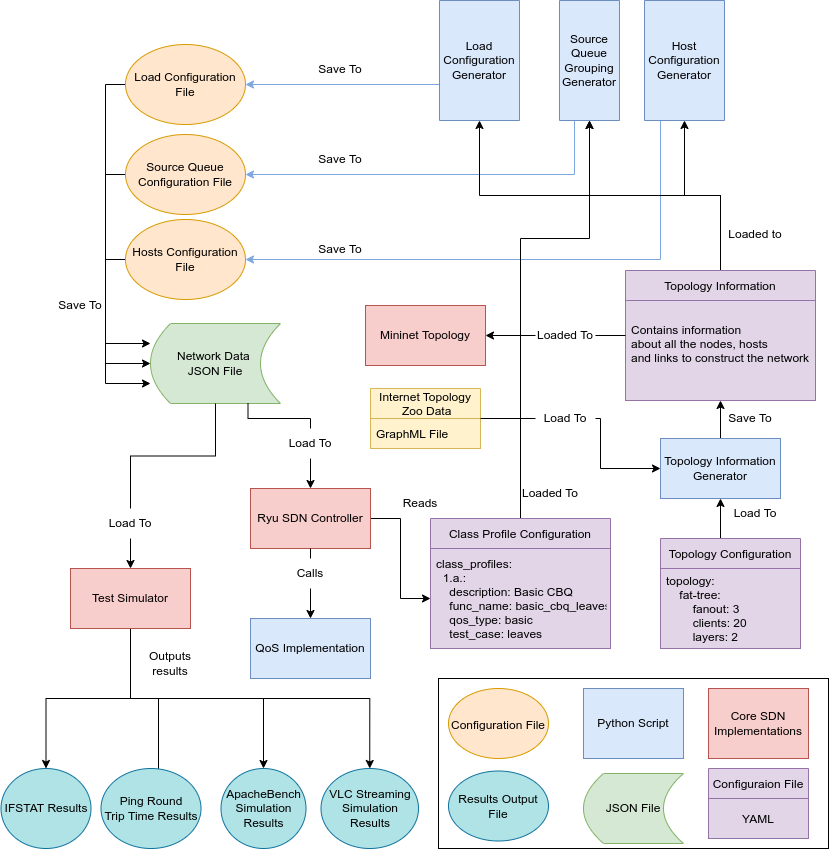
\includegraphics[width=\textwidth]{Figures/Test Framework Architecture.drawio.png}
    \caption{The architecture of the Modified QoS Testing Framework}
    \label{fig:new_architecture}
\end{figure}

The framework is further modified so that the Ryu Controller script now uses the STP protocol to decide the paths of the packets in the topologies, since typical topologies like the mesh and real-life data from the ITZ contain loops for better network resiliency \cite{smith_shortest_2011}. The reference \textsc{simple\_switch\_stp\_13.py} code from the Ryu Library is used as a basis to develop the controller that will run on any topology and with any QoS queue management technique.

Finally, we simplify the framework so that the framework no longer needs pickle files to specify the QoS Implementations. Instead, the Ryu Controller directly calls the appropriate QoS Implementation according to the algorithm specified by the \textit{Class Profile Configuration} file. The modified framework is installed on a system configured as described in Figure \ref{fig:tools}. Software in the \textit{SDN Simulation} box are used for simulating the networks and running the tests, while the tools in the \textit{Topology Processing} box are used for selecting, diagramming, and processing the various topologies.

\begin{figure}[htbp]
    \centering
    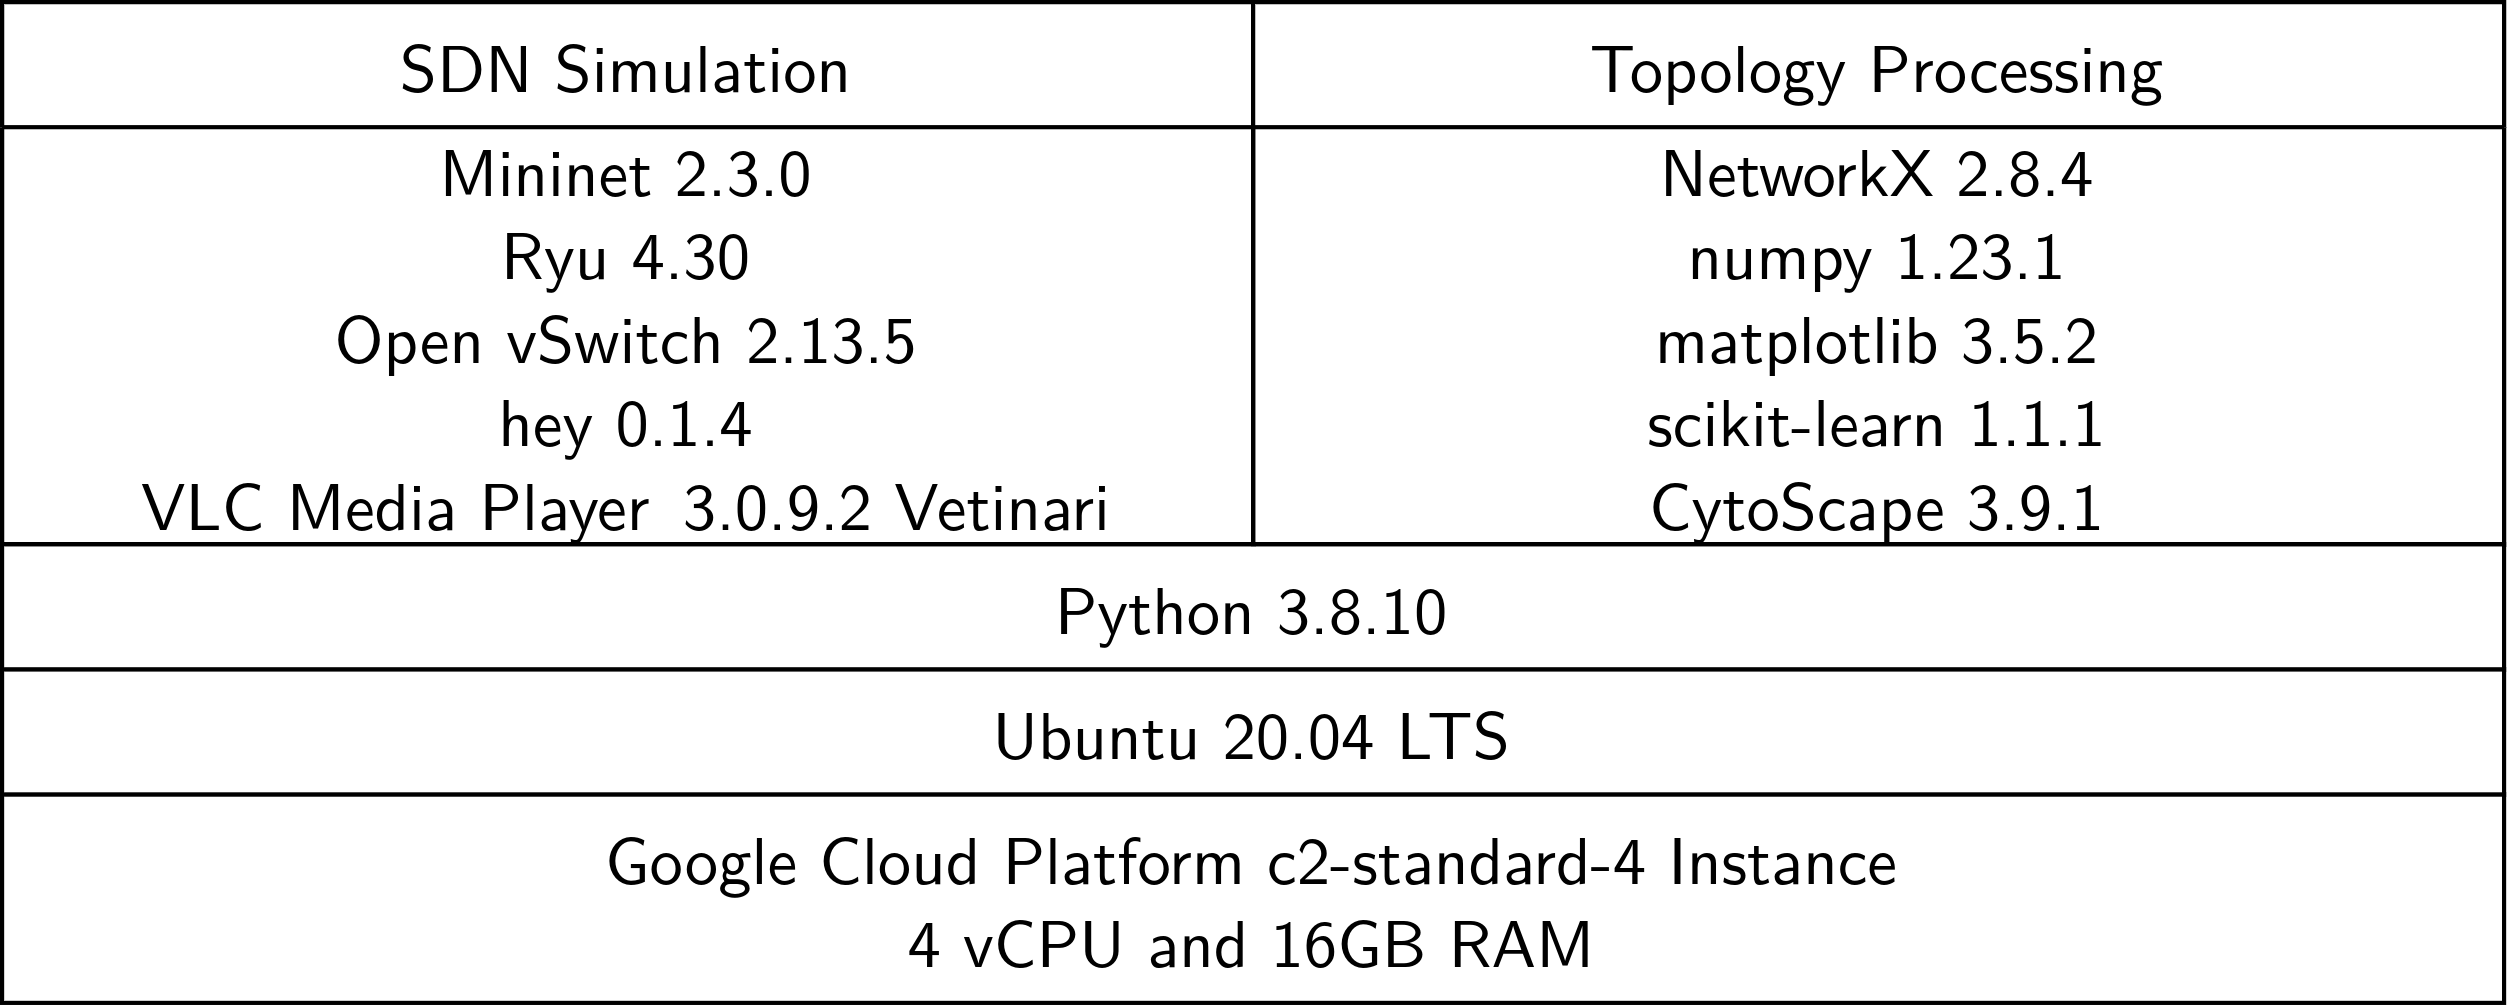
\includegraphics[width=\textwidth]{Figures/Test Machine Configuration.drawio.png}
    \caption{The machine configuration and software tools used in the experiment}
    \label{fig:tools}
\end{figure}

\section{Selected Networks for Testing}
We test the following topologies:
\begin{enumerate}
    \item Fat-tree topology with two layers and fan-out 3 (Figure \ref{fig:BalancedTree})
    \item Hypercube topology with 8 vertices (Figure \ref{fig:Hypercube})
    \item Complete Mesh topology with 5 vertices in the mesh (Figure \ref{fig:CompleteMesh})
    \item Topology from the Internet Topology Zoo, Regional or Country data with less than 40 nodes
\end{enumerate}

The choice of topologies from the Internet Topology Zoo is based on two features: the number of nodes and the number of edges (links) in the graph. From the dataset in the ITZ, we have 133 topologies that are either regional or country data that has less than 40 nodes. This limit is due to the limited resources of the machine that runs the simulations. The clustering was done by reading all 133 topologies into NetworkX, extracting the number of nodes and edges, and using the \textsc{scikit-learn} KMeans clustering library. Each node-edge data point was given the same weight \cite{pedregosa_scikit-learn_2011}. Centroid selection seed was fixed as $0$. We chose 10 random topologies from the four clusters with NumPy, proportional to the number of topologies in each group. The list of the chosen topologies are shown in Table \ref{tab:choices}.

\begin{figure}[htbp]
    \centering
    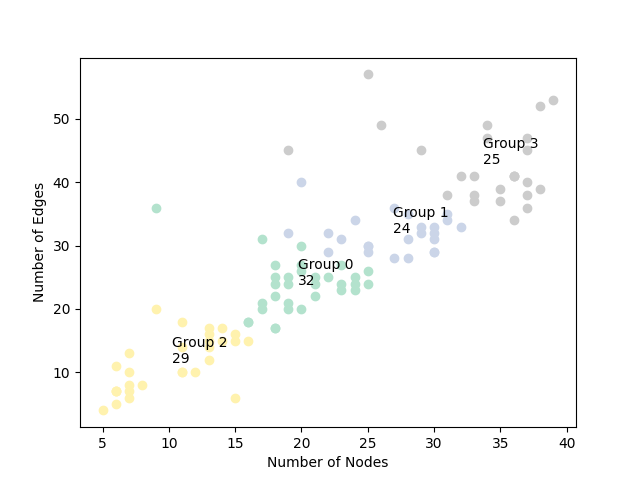
\includegraphics[width=\textwidth]{Figures/clusters.png}
    \caption{133 ITZ topologies as grouped by K-means method based on the number of nodes and number of edges. Numbers in the middle of similarly-colored points indicate the number of topologies in the group.}
    \label{fig:groups}
\end{figure}

\begin{table}[htbp]
    \centering
    \begin{tabular}{ccccc}
    \toprule
        Topology Name & Cluster & \makecell{Number of\\ Nodes} & \makecell{Number of \\Edges} & Location \\
    \midrule
        Saavis (Figure \ref{fig:Saavis}) & 0 & 19 & 20 & USA \\
        Atmnet (Figure \ref{fig:Atmnet})& 0 & 21 & 22 & USA \\
        Ibm (Figure \ref{fig:Ibm})& 0 & 18 & 24 & USA \\
        Agis (Figure \ref{fig:Agis})& 1 & 25 & 30 & USA \\
        WideJpn (Figure \ref{fig:WideJpn})& 1 & 30 & 33 & Japan \\
        Gridnet (Figure \ref{fig:Gridnet})& 2 & 9 & 20 & USA \\
        Nsfnet (Figure \ref{fig:Nsfnet})& 2 & 13 & 15 & USA \\
        Singaren (Figure \ref{fig:Singaren})& 2 & 11 & 10 & Singapore \\
        Janetbackbone (Figure \ref{fig:Janetbackbone})& 3 & 29 & 45 & UK \\
        Canerie (Figure \ref{fig:Canerie})& 3 & 32 & 41 & Canada \\
    \bottomrule
    \end{tabular}
    \caption{10 topologies from the 4 clusters chosen at random with NumPy. Diagrams for these networks are in Appendix I.}
    \label{tab:choices}
\end{table}

In general, we have selected topologies of various sizes, some with many loops, and some with structures that are more tree-like. Although this only simulates networks with less than 40 nodes, the variety of network structure and sizes are still evident in the samples.

\section{Topology Configuration}
To implement the topologies within the context of the simulations, we take the fat-tree topology from the original study by Regencia and Yu and modify the number, arrangement, and links in the switches that connect the ``core'' switch to the clients. The ``core'' switch is the switch that connects to a switch connecting all servers in a star topology formation. In Figure \ref{fig:original_topology}, the topology to be changed corresponds to the circled switches.

\begin{figure}[htbp]
    \centering
    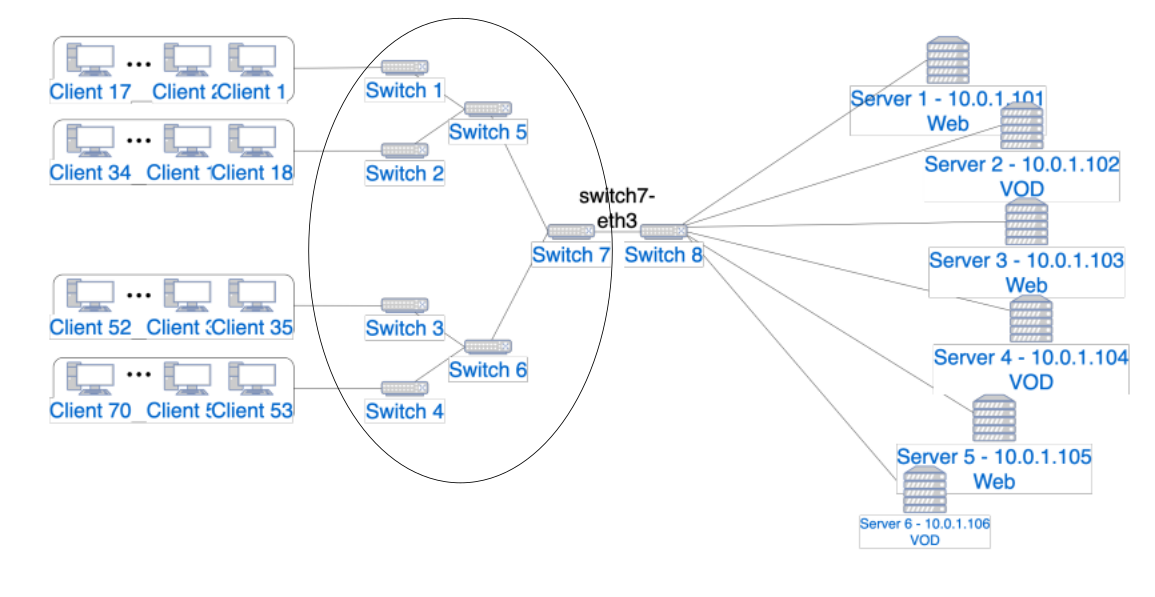
\includegraphics[width=\textwidth]{Figures/original_topology.png}
    \caption{Diagram of a fat-tree topology tested in Regencia and Yu}
    \label{fig:original_topology}
\end{figure}

The ``core'' switch in the fat-tree topology remains to be the root switch of the tree. In the complete mesh topology and the hypercube, the node with the numerical label $0$ is considered to be the root switch, since the topologies has at least one symmetry with respect to any node in the mesh. For the topologies from the Internet Topology Zoo, we simulate the worst case scenario by assigning the core as the node with the highest number of total hops from all other nodes, which is calculated with the Floyd-Warshall algorithm provided by the NetworkX library.

Clients are placed on all ``leaf'' switches, or switches furthest away from the ``core'' switch, which are switches that have the longest path from the core switch in the graph that represents the topology. As an exception, the fat-tree topology will have clients connected to its explicit leaf switches. The clients will be distributed equally among the switches. Finally, we will connect four servers to the server switch to complete the topology. The diagrams of the tested topologies are included in Appendix I.

Links will be configured with their default setting of 10Gbps in Mininet, as in the previous study. Although real-life networks do not behave this way, the ITZ data is not complete to simulate the link speeds.

\section{Server Configuration}
There will be 2 servers running a Python server from the http.server library, and 2 servers running a VLC streaming server using the Real Time Streaming Protocol. Table \ref{tab:httpserverconfig} shows the files hosted by the HTTP servers, and Table \ref{tab:vlcconfig} shows the videos hosted by the VLC servers.

\begin{table}[htbp]
    \centering
    \begin{tabular}{cccc}
        \toprule
        \multirow{2}{*}{Server ID} & \multirow{2}{*}{Server IP Address} & \multicolumn{2}{c}{File Size and Type} \\
         &  & Low Load & High Load \\
        \midrule
        Server 1 & 10.0.1.101 & \qty{100}{\kilo \byte} JPEG & \qty{10}{\mega \byte} JPEG \\
        Server 3 & 10.0.1.103 & \qty{16}{\mega \byte} PDF & \qty{100}{\mega \byte} PDF  \\
        \bottomrule
    \end{tabular}
    \caption{Files hosted by the two Python http.server servers}
    \label{tab:httpserverconfig}
\end{table}

\begin{table}[htbp]
    \centering
    \begin{tabular}{cccc}
        \toprule
        \multirow{2}{*}{Server ID} & \multirow{2}{*}{Server IP Address} & \multicolumn{2}{c}{Video Resolution} \\
         &  & Low Load & High Load \\
        \midrule
        Server 2 & 10.0.1.102 & 360p & 480p \\
        Server 4 & 10.0.1.104 & 480p & 720p  \\
        \bottomrule
    \end{tabular}
    \caption{Files hosted by the two VLC RTSP servers}
    \label{tab:vlcconfig}
\end{table}

\section{Client Configuration}
There will be 48 clients that will simultaneously run an ApacheBenchmark test and a VLC client. Each client will request for different files from the server, and every file in each server will get requests as equally as possible. Table \ref{tab:clientconfig} shows the configuration of these clients.

\begin{table}[htbp]
    \centering
    \begin{tabular}{ccc}
    \toprule
        Client numbers & Server & Load\\
    \midrule
        \multirow{2}{*}{$1, 5, 9, 13, \dots 41, 45$}  & Server 1 & Low \\
        & Server 2 & Low \\ \hline
        \multirow{2}{*}{$2, 6, 10, 14, \dots 42, 46$}  & Server 3 & Low \\
        & Server 4 & Low \\ \hline
        \multirow{2}{*}{$3, 7, 11, 15, \dots 43, 47$}  & Server 1 & High \\
        & Server 2 & High \\ \hline
        \multirow{2}{*}{$4, 8, 12, 16, \dots 44, 48$}  & Server 3 & High \\
        & Server 4 & High \\
    \bottomrule
    \end{tabular}
    \caption{Configurations for clients denoting the server and the load that the client will request in the simulations}
    \label{tab:clientconfig}
\end{table}

\section{Quality of Service configuration}
All ports in a subset of switches in the network will have QoS paremeters applied to them with the \texttt{ovs-ofctl} command. In the case of leaf-enforced QoS, the parameters were applied to all ports at the switches that are connected to the clients. In the case of core-enforced QoS, they were applied at the port connecting the core switch to the server switch. Table \ref{tab:CBQconfig} and \ref{tab:SBQconfig} shows the QoS configuration used for CBQ and SBQ respectively.

\begin{table}[htbp]
    \centering
    \begin{tabular}{ccccc}
    \toprule
        Queue number & Traffic Protocol & Application & \thead{Minimum and \\Maximum bandwidth} & Priority\\
    \midrule
        $Q_0$ & TCP & HTTP traffic (PDF, JPEG files) & \qty{333.33}{\mega \bit / \second} & 1 \\
        $Q_1$ & UDP & Video streaming & \qty{333.33}{\mega \bit / \second} & 2 \\
        $Q_2$ & Others(ICMP, ARP) & Network control & \qty{333.33}{\mega \bit / \second} & 0 \\
    \bottomrule
    \end{tabular}
    \caption{QoS configuration used to implement simple CBQ QoS enforcement}
    \label{tab:CBQconfig}
\end{table}

\begin{table}[htbp]
    \centering
    \begin{tabular}{cccc}
    \toprule
        Queue number & Source & \thead{Minimum and \\Maximum bandwidth} & Priority\\
    \midrule
        $Q_0$ & 10.0.0.1, 4, 7 ... & \qty{333.33}{\mega \bit / \second} & 1 \\
        $Q_1$ & 10.0.0.2, 5, 8 ... & \qty{333.33}{\mega \bit / \second} & 2 \\
        $Q_2$ & 10.0.0.3, 6, 9 ... & \qty{333.33}{\mega \bit / \second} & 0 \\
    \bottomrule
    \end{tabular}
    \caption{QoS configuration used to implement Source-based CBQ QoS enforcement}
    \label{tab:SBQconfig}
\end{table}

\section{Network Simulation and Testing} \label{3:testing}
The methodology of testing the networks is similar to Chato and Yu \cite{chato_exploration_2016} which is also used in Regencia and Yu \cite{yang_introducing_2022}. Since the modified framework uses STP, we have to wait for the STP to converge before running the rest of the tests. We first run pings until a successful ping has been executed. We measure the time for this to take for all topologies. Then, for the actual tests, we wait for at least this amount of time before executing the rest of the tests.

For every topology, we run \texttt{ping} tests, \texttt{ifstat}, \texttt{hey}, and VLC Streaming under all the QoS algorithms to be tested. We show the exact process of running the benchmarks in Figure \ref{fig:benchmark}.

\begin{figure}
    \centering
    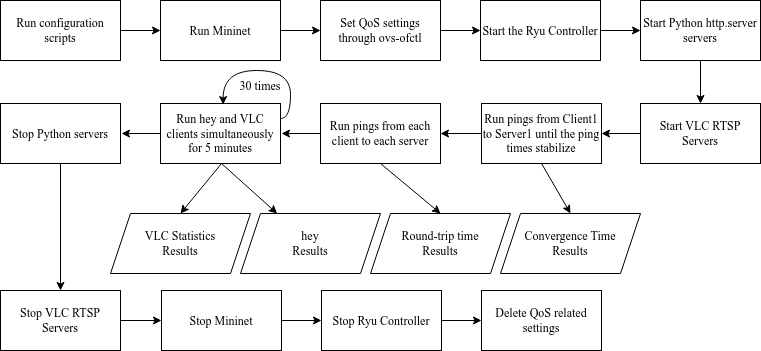
\includegraphics[width=\textwidth]{Figures/Test Procedure.drawio.png}
    \caption{The procedure for running the benchmarks}
    \label{fig:benchmark}
\end{figure}

One key difference between this methodology and the methodology from Regencia and Yu is that different topologies take different amounts of time for the switches in the network to install flows. We define the \textit{convergence time} as the time it takes for pings to go consistently under 1 second after the STP established proper connections between the servers and the clients. Yoo and Yu have shown that the convergence time is different for different types of topologies \cite{yoo_building_2022}. Therefore, this characteristic is measured first before running other tests.

\chapter{RESULTS}
We discuss the convergence times, round-trip times, HTTP stress test benchmark results, and video streaming benchmark results in order, comparing the performances of the different network topologies under the two queuing algorithms tested.

\section{Convergence times}
First, we discuss the convergence time as described in section \ref{3:testing}. Table \ref{tab:convergence} shows the convergence times of the tested topologies. In both the Basic and Source CBQ, in general, larger networks exhibited higher convergence times. The simple class--based queuing algorithm took much longer to converge than the source class-based queuing algorithm in this test.

\begin{table}[htbp]
    \centering
    \begin{tabular}{cccc}
        \toprule
        \multirow{2}{*}{Topology} & \multirow{2}{*}{Network size}& \multicolumn{2}{c}{Convergence Times} \\
        & & Basic CBQ & Source CBQ \\
        \midrule \\

        Agis & 5.370 & 3.950 & \\
        Atmnet & 6.323 & 3.649 & \\
        Canerie & 4.640 & 5.118 & \\
        Gridnet & 3.772 & 3.987 & \\
        Ibm & 3.669 & 4.074 & \\
        Janetbackbone & 3.532 & & \\
        Nsfnet & 3.684 & 4.003 & \\
        Savvis & 3.139 & 3.107 & \\
        Singaren & 3.490 & 3.669 & \\
        WideJpn & 3.848 & 4.074 & \\
        Mesh & 3.047 & 3.671 & \\
        Tree & 3.605 & 3.613 & \\
        \bottomrule
    \end{tabular}
\end{table}

\section{Round-trip times}
Next, we discuss the round trip times after the network has converged. The round trip times are similar in both algorithms, as shown in Tables \ref{tab:cbq_pings} and \ref{tab:sbq_pings}.

\section{VLC traffic performance}

\section{HTTP traffic performance}


\chapter{CONCLUSION}
\section{Conclusions}
We were able to modify the testing framework to properly accomodate different topologies through the use of the NetworkX library and a simple modification to the Ryu switch algorithm with the Spanning-Tree Protocol.

From the results we provide the following conclusions:
\begin{enumerate}
    \item For round trip times, the two topologies showed similar results; however, the Basic CBQ was able to provide for better service in video traffic, which was the priority traffic in the experiment.
    \item For HTTP file transfer performance, while Basic CBQ was more reliable, with little to no failed requests, raw file transfer rate was higher for Source CBQ in some topologies. 
    \item The performance characteristics across topologies was not purely dependent on the network size. The shape and structure of the topology can also affect the performance metrics.
    \item In Source CBQ, the difference of performance between the different clusters was more pronounced in the two benchmarks, while in Basic CBQ, the trend of increasing performance when moving to smaller-sized clusters was less clear.
    \item Overall, Basic CBQ outperformed Source CBQ in the random sample of ITZ network topologies, as well as the two model topologies selected for testing. 
\end{enumerate}
Regarding point 4, this implies that Basic CBQ was more consistent across all topologies in the video streaming benchmark, which means that Basic CBQ exhibited better performance than Source CBQ.

\section{Recommendations}
The following improvements to this research can be implemented to better understand the behavior of the QoS algorithms in different networks:
\begin{enumerate}
    \item Increase the number of servers and the variety of traffic
    \item Incorporate PCAP into this research to simulate real-life traffic better
    \item Use different path-resolution algorithms other than STP
    \item Increase the scale, both in the size of the network and the number of clients
    \item Investigate algorithms aside from Basic CBQ and Source CBQ, and investigate the differences between leaf-enforced and source-enforced algorithms
    \item Investigate the effect of graph structure and shape, while controlling for the number of nodes.
\end{enumerate}



\printbibliography
\addappheadtotoc

\begin{appendices}

\chapter{Diagrams of Topologies}
This appendix contains diagrams of the topologies to be tested, configured according to Section 3.2. The networks were visualized with CytoScape \cite{shannon_cytoscape_2003}. Unless specified, the topologies are from the Internet Topology Zoo. In all diagrams, Green nodes are servers, Purple nodes are clients, and Orange nodes are switches.
\begin{figure}
    \centering
    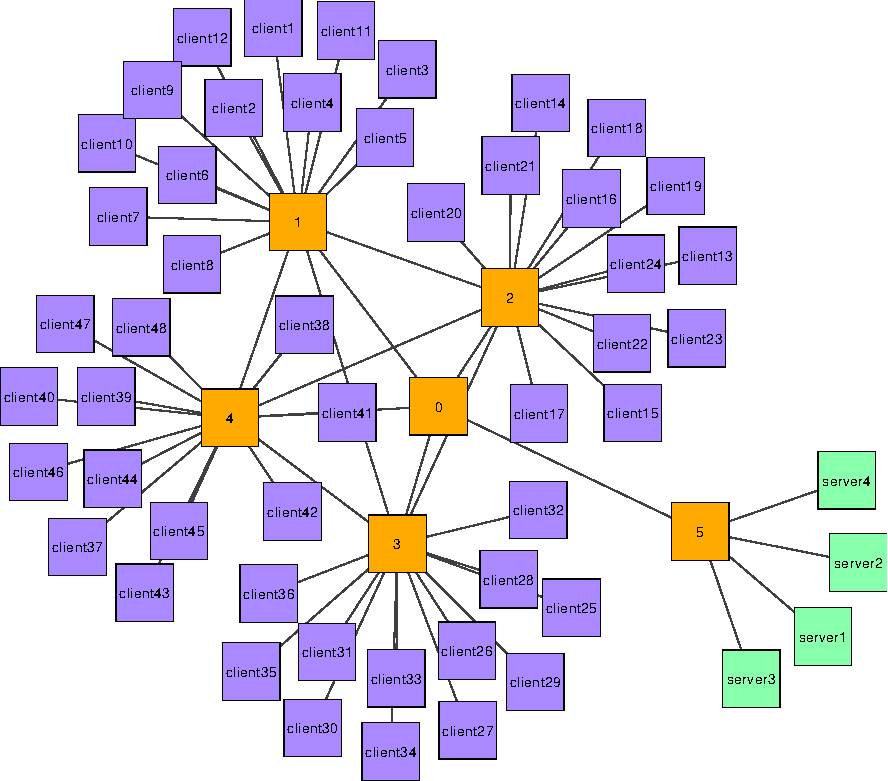
\includegraphics[width=\linewidth]{Networks/Complete Graph_final.pdf}
    \caption{Complete Mesh Topology with 5 nodes in the mesh}
    \label{fig:CompleteMesh}
\end{figure}

\begin{figure}
    \centering
    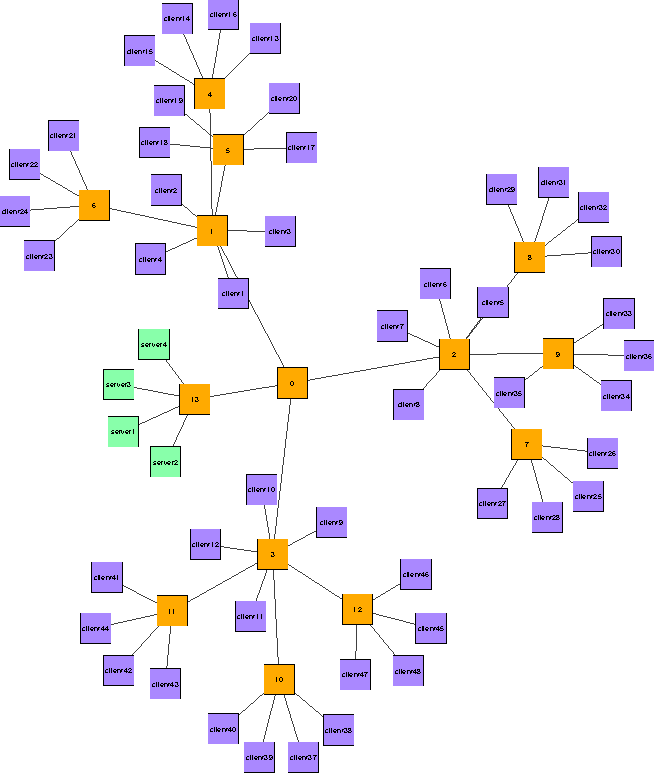
\includegraphics[width=\linewidth]{Networks/Balanced Tree_final.pdf}
    \caption{Fat-Tree Topology with fanout 3 and height 2}
    \label{fig:BalancedTree}
\end{figure}

\begin{figure}
    \centering
    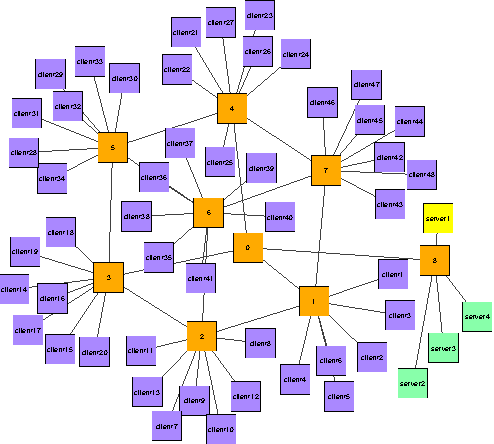
\includegraphics[width=\linewidth]{Networks/Hypercube_final.pdf}
    \caption{Hypercube Topology with 8 nodes and 12 edges}
    \label{fig:Hypercube}
\end{figure}

\begin{figure}[htbp]
    \centering
    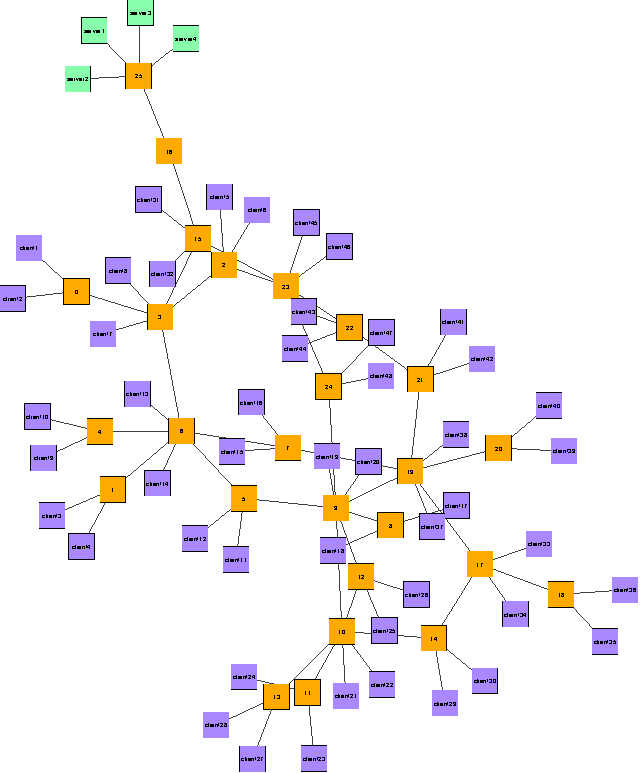
\includegraphics[width=\linewidth]{Networks/Agis_final.pdf}
    \caption{Agis Topology}
    \label{fig:Agis}
\end{figure}

\begin{figure}[htbp]
    \centering
    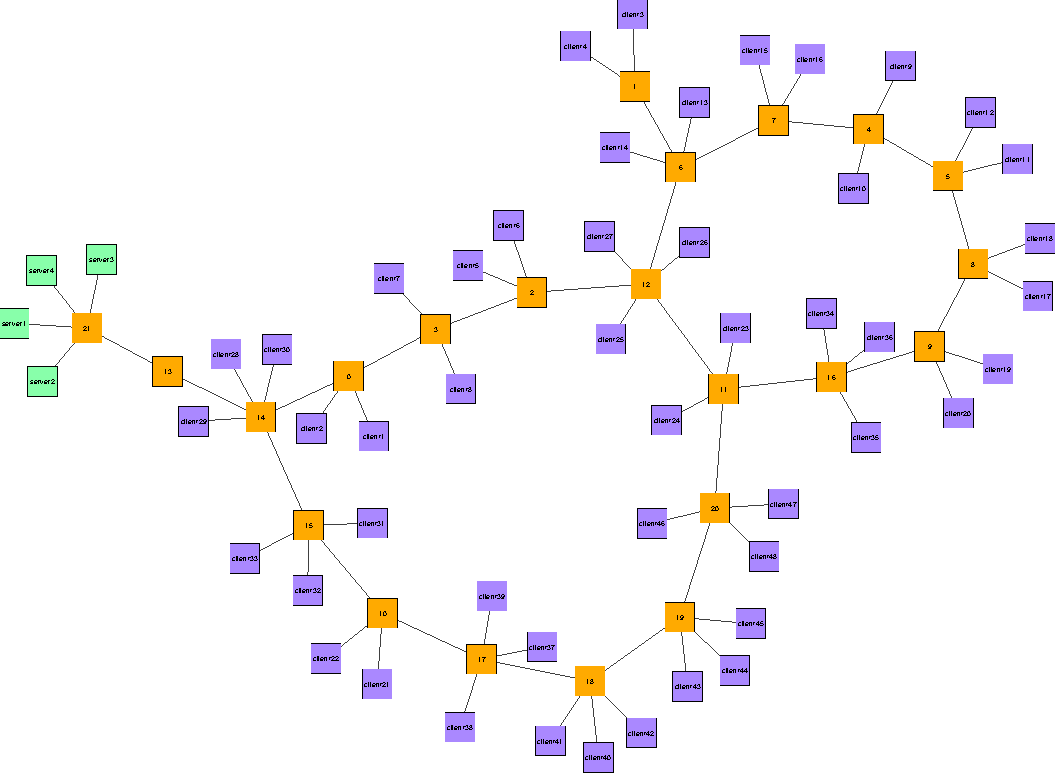
\includegraphics[width=\linewidth]{Networks/Atmnet_final.pdf}
    \caption{Atmnet Topology}
    \label{fig:Atmnet}
\end{figure}

\begin{figure}[htbp]
    \centering
    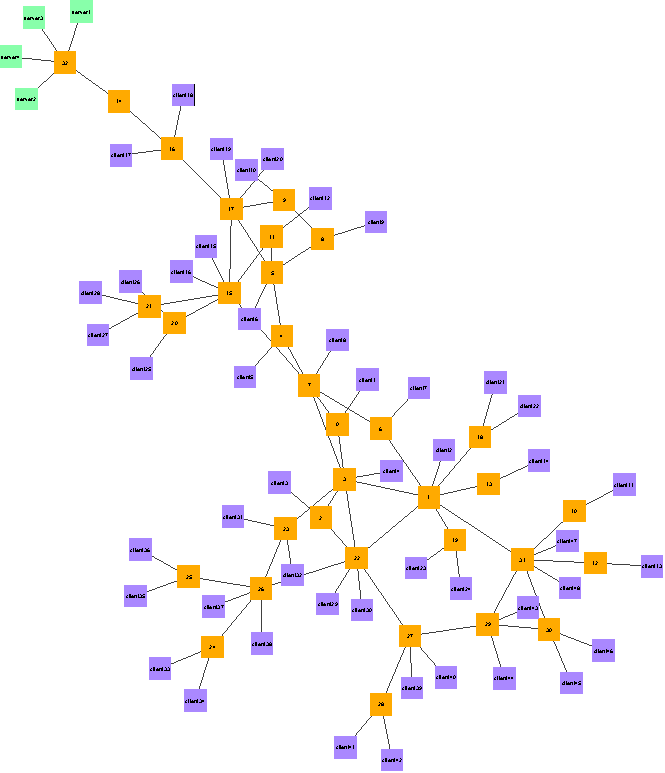
\includegraphics[width=\linewidth]{Networks/Canerie_final.pdf}
    \caption{Canerie Topology}
    \label{fig:Canerie}
\end{figure}

\begin{figure}[htbp]
    \centering
    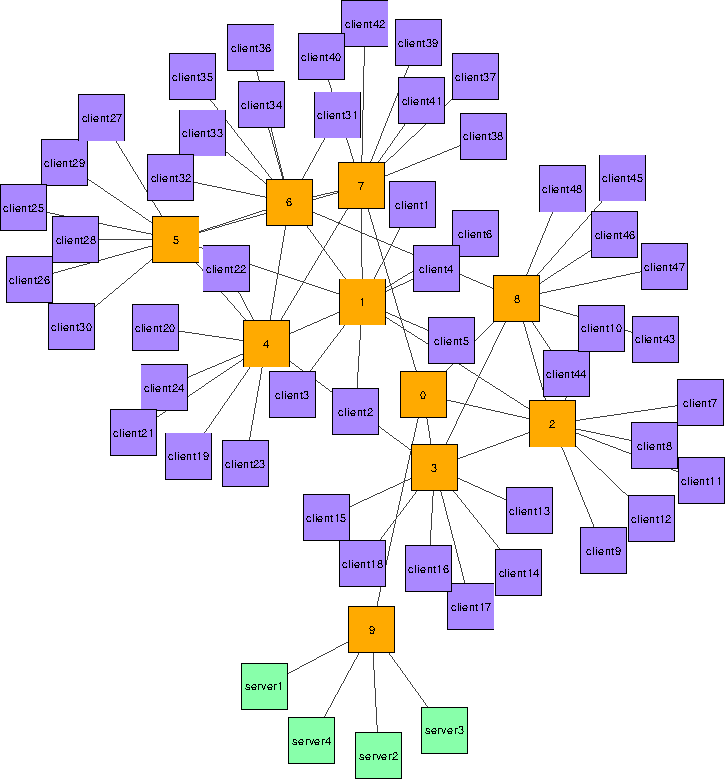
\includegraphics[width=\linewidth]{Networks/Gridnet_final.pdf}
    \caption{Gridnet Topology}
    \label{fig:Gridnet}
\end{figure}

\begin{figure}[htbp]
    \centering
    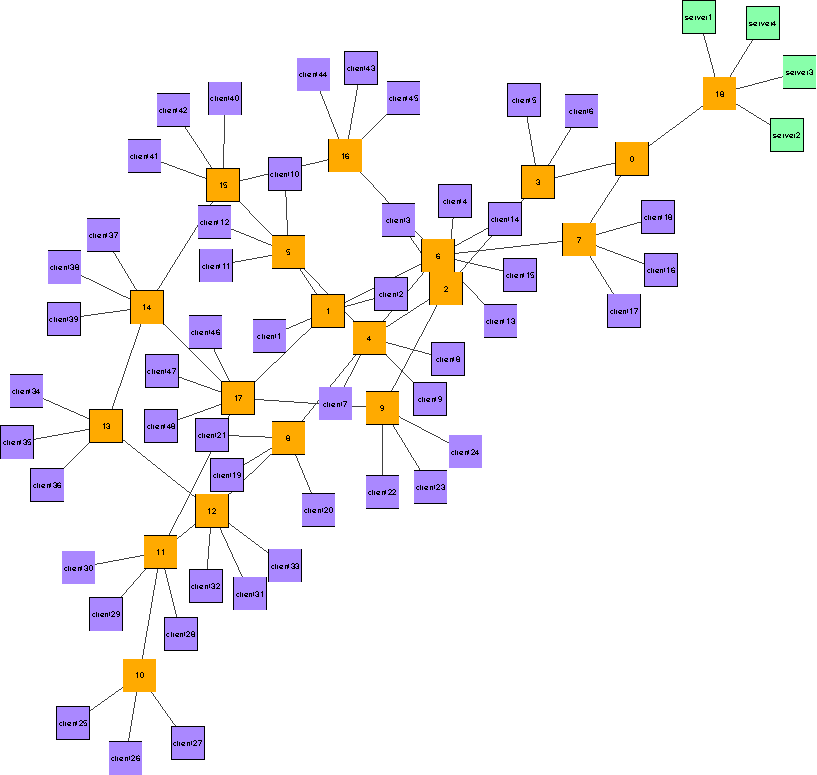
\includegraphics[width=\linewidth]{Networks/Ibm_final.pdf}
    \caption{Ibm Topology}
    \label{fig:Ibm}
\end{figure}

\begin{figure}[htbp]
    \centering
    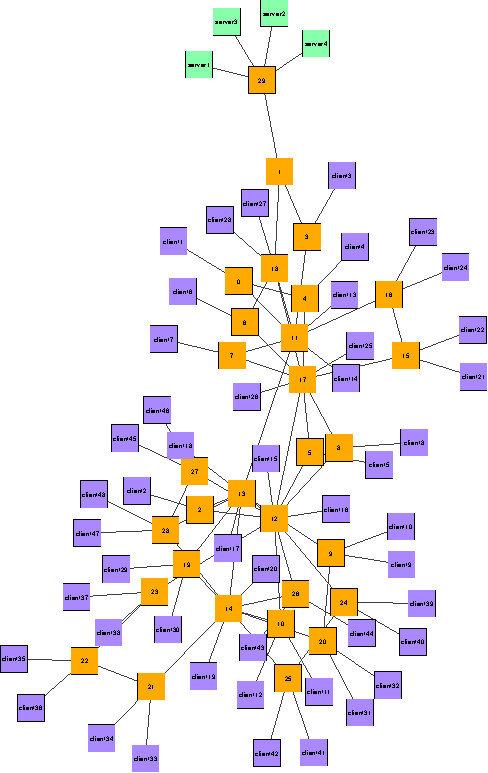
\includegraphics[width=\linewidth, height=\textheight]{Networks/Janetbackbone_final.pdf}
    \caption{Janetbackbone Topology}
    \label{fig:Janetbackbone}
\end{figure}

\begin{figure}[htbp]
    \centering
    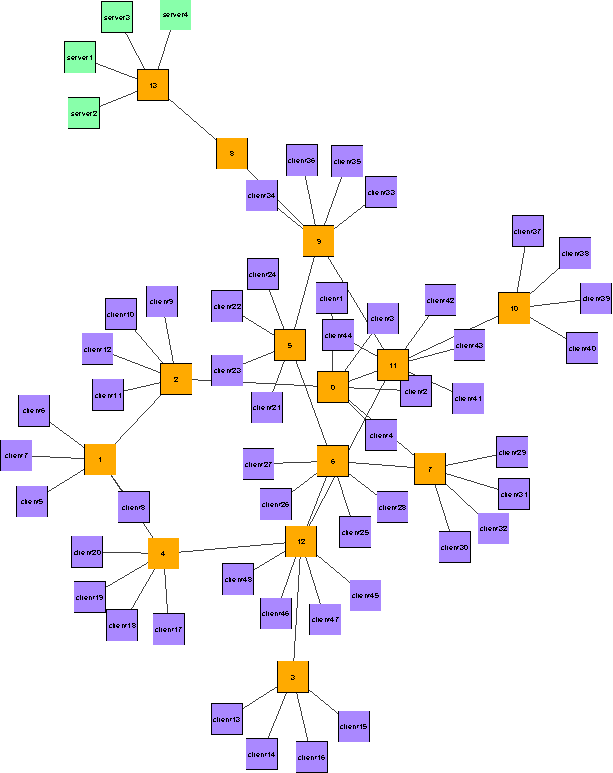
\includegraphics[width=\linewidth]{Networks/Nsfnet_final.pdf}
    \caption{Nsfnet Topology}
    \label{fig:Nsfnet}
\end{figure}

\begin{figure}[htbp]
    \centering
    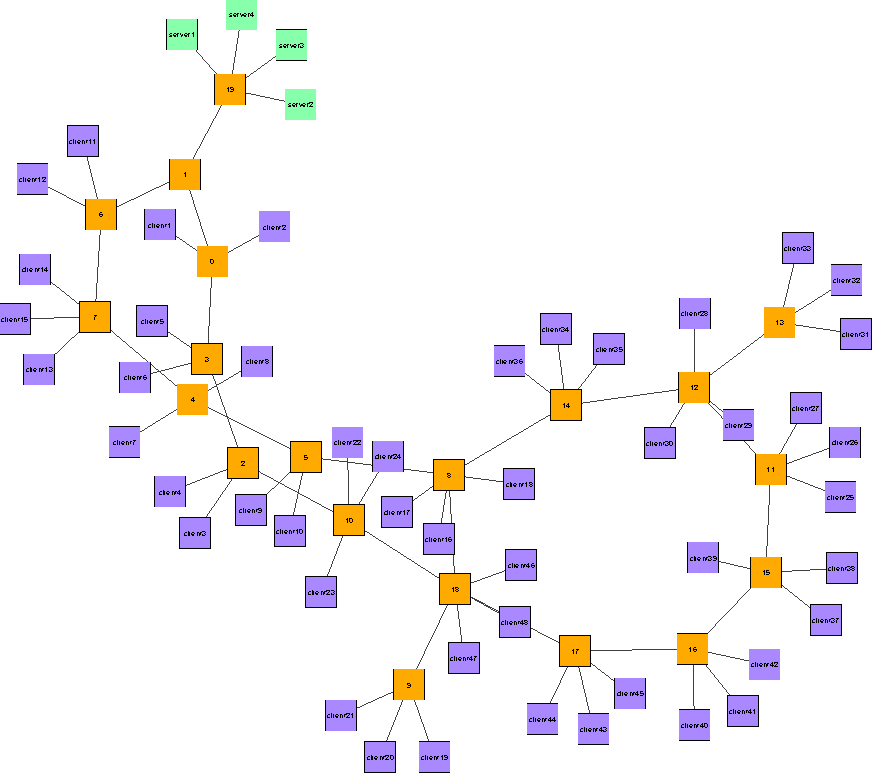
\includegraphics[width=\linewidth]{Networks/Savvis_final.pdf}
    \caption{Savvis Topology}
    \label{fig:Saavis}
\end{figure}

\begin{figure}[htbp]
    \centering
    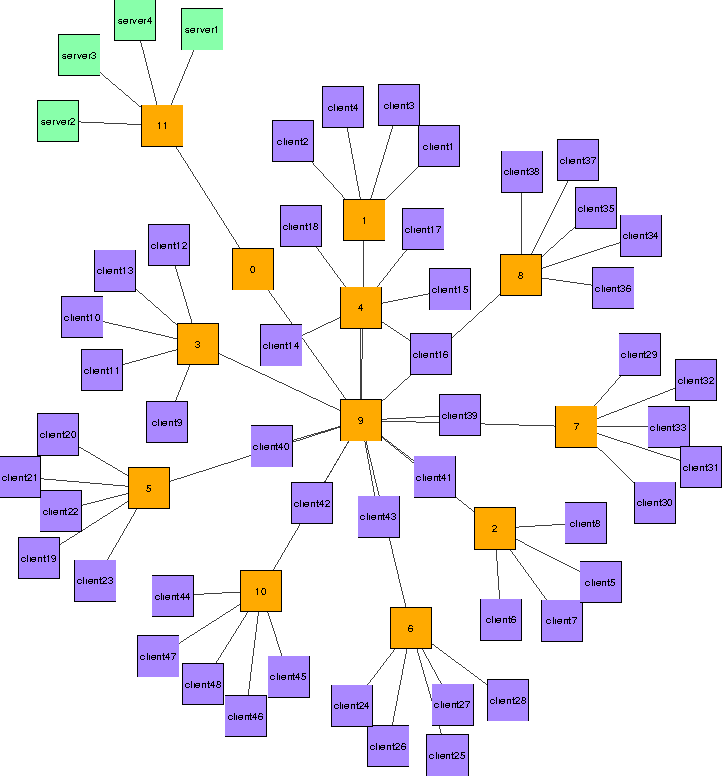
\includegraphics[width=\linewidth]{Networks/Singaren_final.pdf}
    \caption{Singaren Topology}
    \label{fig:Singaren}
\end{figure}

\begin{figure}[htbp]
    \centering
    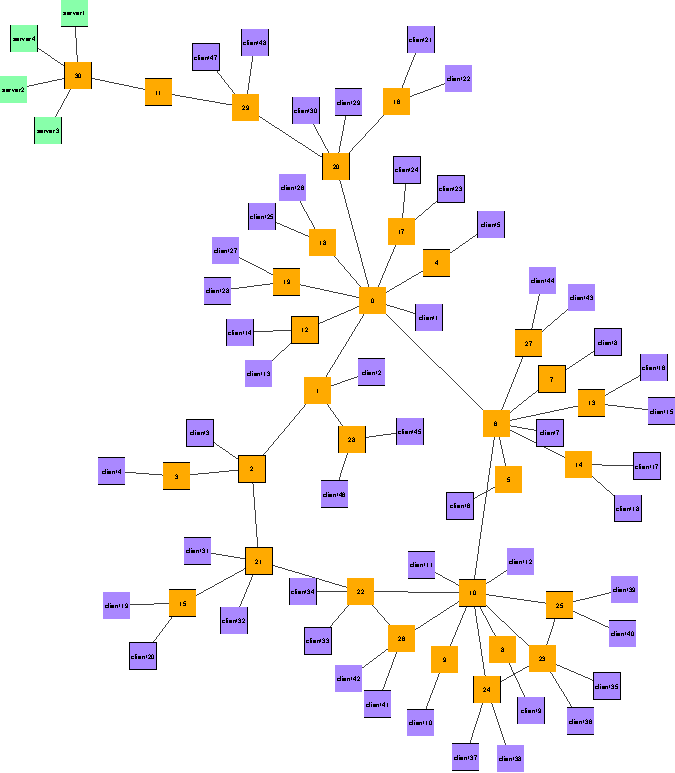
\includegraphics[width=\linewidth]{Networks/WideJpn_final.pdf}
    \caption{WideJpn Topology}
    \label{fig:WideJpn}
\end{figure}
\chapter{Paper submitted to the 2022 Inernational Conference on Engineering and Emerging Technologies, Kuala Lumpur, Malaysia}
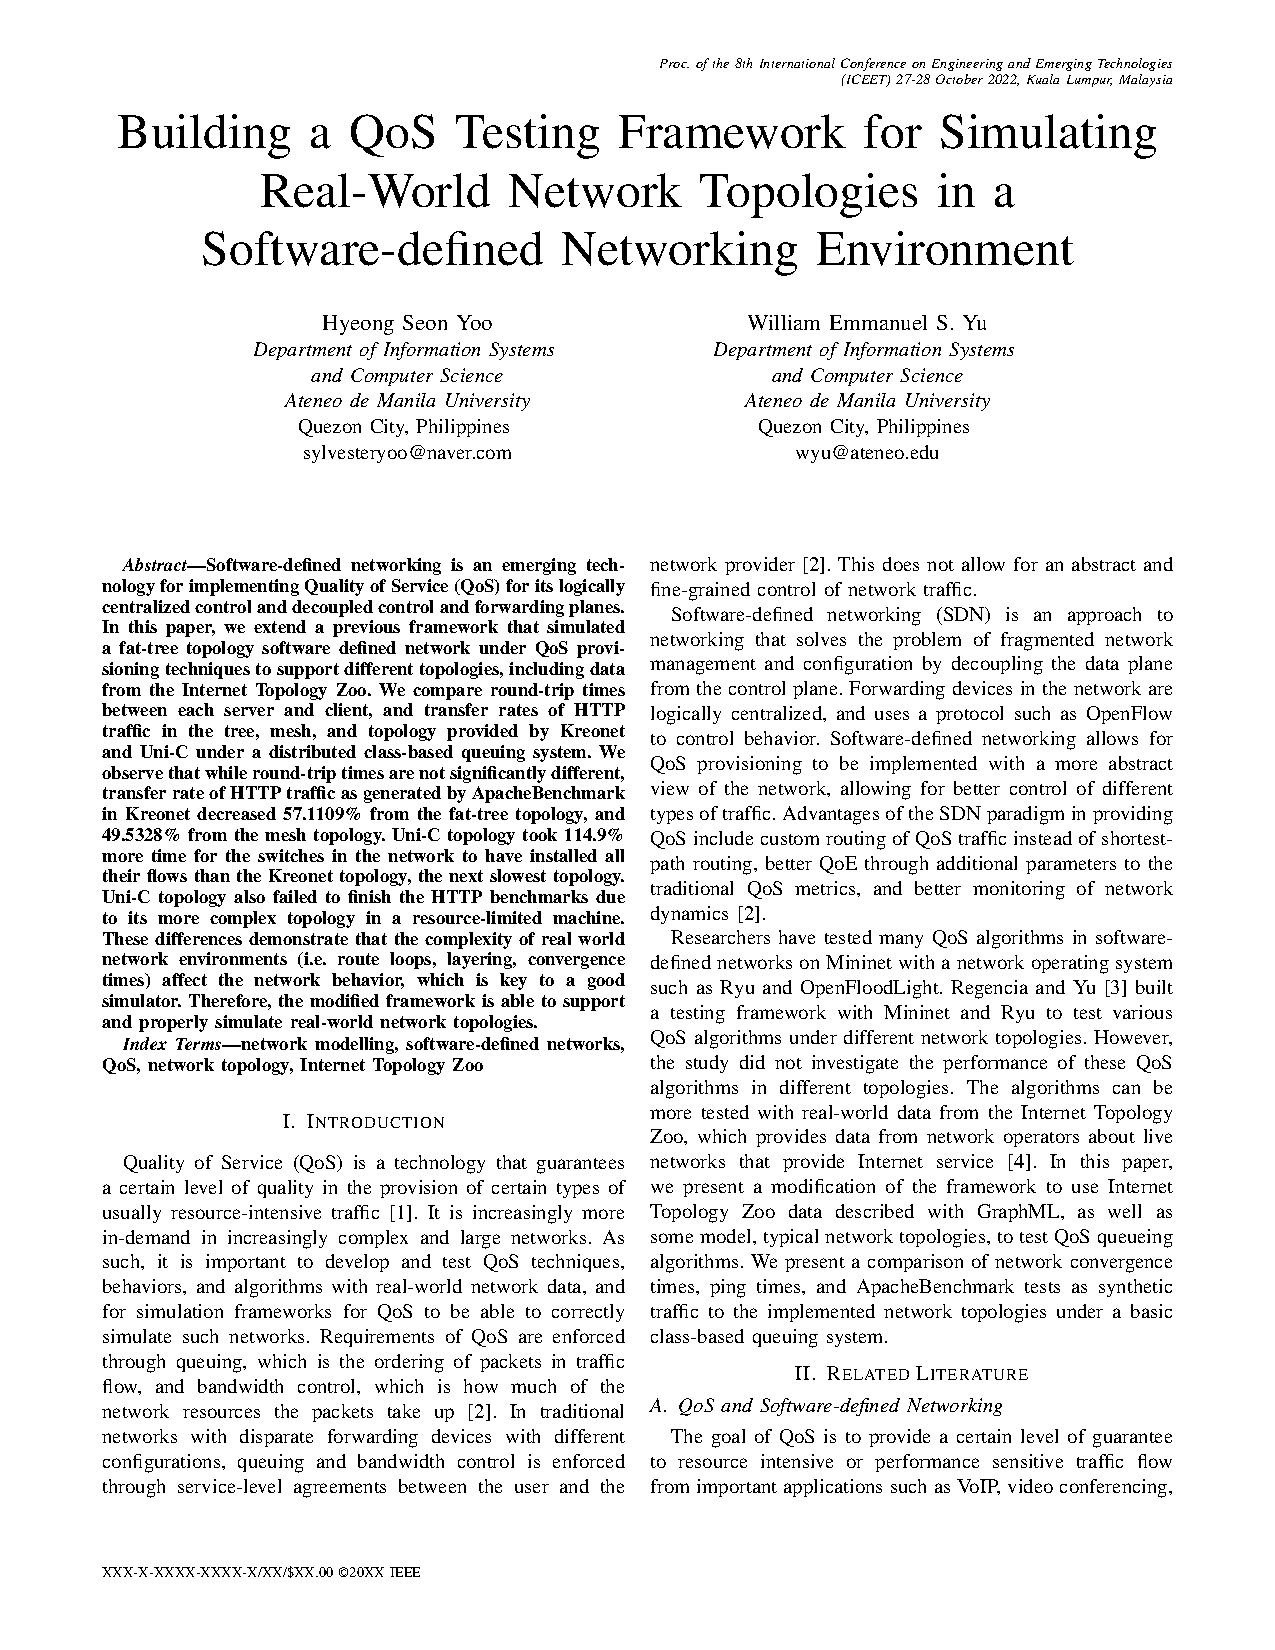
\includepdf[pages=-]{Conference_Building_Framework.pdf}

\chapter{Paper submitted to the 2023 Fourth International Conference on Frontiers of Computers and Communication, Xiamen, China}
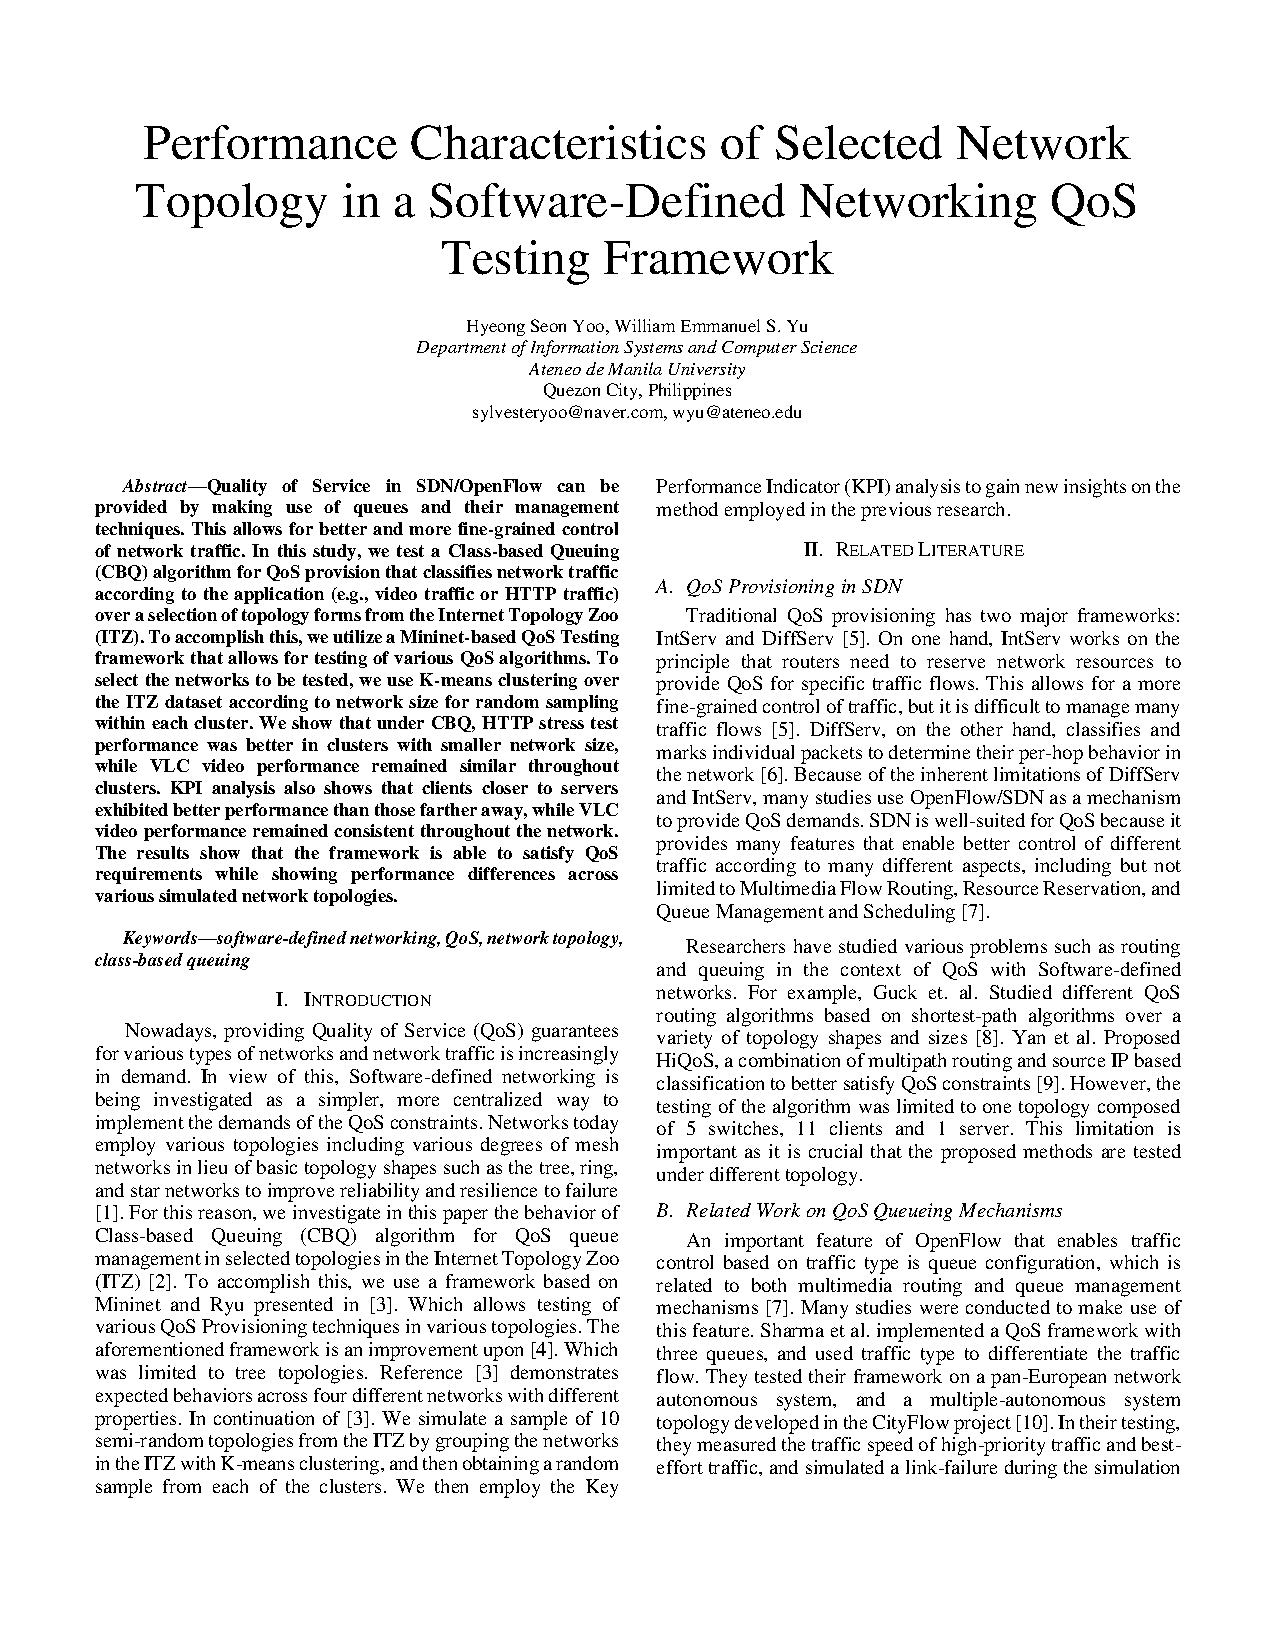
\includepdf[pages=-]{JA-0008-12.24.pdf}
\end{appendices}

\end{document}
